% !TeX spellcheck = en_GB
\chapter{\IfLanguageName{dutch}{Stand van zaken}{State of the art}}
\label{ch:stand-van-zaken}

% Tip: Begin elk hoofdstuk met een paragraaf inleiding die beschrijft hoe
% dit hoofdstuk past binnen het geheel van de bachelorproef. Geef in het
% bijzonder aan wat de link is met het vorige en volgende hoofdstuk.

This chapter contains the state of affairs. As mentioned in the introduction this part of the bachelor's thesis will be used to get an in-depth understanding of the four key themes that incorporate the changes in Windows Server 2019. First, for the key themes mentioned before, a basic understanding of what they are will be established together with how these have been implemented in the latest version of the \acrshort{os}.

%Dit hoofdstuk bevat je literatuurstudie. De inhoud gaat verder op de inleiding, maar zal het onderwerp van de bachelorproef *diepgaand* uitspitten. De bedoeling is dat de lezer na lezing van dit hoofdstuk helemaal op de hoogte is van de huidige stand van zaken (state-of-the-art) in het onderzoeksdomein. Iemand die niet vertrouwd is met het onderwerp, weet er nu voldoende om de rest van het verhaal te kunnen volgen, zonder dat die er nog andere informatie moet over opzoeken \autocite{Pollefliet2011}.
%\textcite{Knuth1998} schreef een van de standaardwerken over sorteer- en zoekalgoritmen. Experten zijn het erover eens dat cloud computing een interessante opportuniteit vormen, zowel voor gebruikers als voor dienstverleners op vlak van informatietechnologie~\autocite{Creeger2009}.

% Pas na deze inleidende paragraaf komt de eerste sectiehoofding.
\section{Hybrid cloud}

Hybrid Cloud is a topic that has gained more momentum over the past years. This makes it a consistent topic of interest for organizations and makes it one of the keystone themes in Windows Server 2019. \autocite{MWST2018} It is with this in mind that it is an essential part of the bachelor's thesis. It is especially beneficial to know the advantages on this aspect of Windows Server since the latest version and how these improve workflow and how these can be leveraged by organizations, in particular, Delaware.

\subsection{Types of cloud solutions}

The National Institute of Standards and Technology differentiates four types of clouds \autocite{Mell2011}:
\begin{itemize}
	\item Private Cloud
	\item Community Cloud
	\item Public Cloud
	\item Hybrid Cloud
\end{itemize}	

%TODO Usage of types of clouds in a business environment
%Poll op LinkedIn

\subsubsection{Private cloud}
A private cloud is an internal infrastructure in the cloud that is designated for usage by a single organization, that can consist of multiple clients, albeit in the same organization. It is only accessible inside a private internal network or over the Internet for a selected amount of users instead than for the general public. It can also be known by other names such as internal or corporate cloud. Private clouds main advantage is the higher level of security and privacy they offer for organizations through the usage of in-house hosted infrastructure and additional company firewalls. The biggest disadvantage that comes with this added layer of security, is the responsibility that is given to the information technology team that manages the private cloud. This means, on top of the additional in-house hosting cost, that they require the same amount of man-hours that come with the management of a traditional datacenter. 
Still the private cloud holds a great benefit compared to long-standing methods. As reported by IBM, which saved more than \$1.5 billion by reducing their number of datacenters from 115 to 5. This is due to the implementation of a private cloud. \autocite{Hofmann2010} 


\subsubsection{Community cloud}
When several organizations collaborate to meet the requirements that are demanded of the IT infrastructure, they are using a community cloud. This means that it can be managed in-house or by a third-party organizations that operates inside the same community. This form of operation tackles one of the main problems of a private cloud, it shares the costs over multiple organizations. Since they are operating inside the same community, they share the same concerns and will be subjected to the same requirements that can be imposed by a governing instance. 
This advantage over private clouds is only a partial improvement. This reduction in cost thanks to the sharing of infrastructure means a reduction in security. This means it is a viable alternative to  organizations that have some security concerns with usage of a public cloud. 
\newline
An example of this is described in an article \autocite{Yao2014} about how small hospitals in China, not all of which can provide their own infrastructure, could utilize a community cloud. These grass-roots healthcare institutions, that are all within the same community, can share the cost and management of this cloud to provide an attractive hospital information solution to improve their service without the extensive cost nor the need for additional security concerns regarding confidential information in patient files.

\subsubsection{Public cloud}
Amazon Web Services, Oracle Cloud and Microsoft Azure are only some examples of public clouds. Most solutions are offered by organizations, like those mentioned above, who manage and operate their datacenter and provide access to their cloud via the Internet. This eliminates the cost that is associated with the management and responsibility of a private cloud, where the IT department is responsible, and thus significantly reduces the cost in same cases. Public cloud also provides the possibility for easy scalability and flexibility in comparison with private clouds, where the hardware needs to be available in-house. This makes it ideal for temporary solutions.
\newline
\textcite{Singh2012} concluded, in a comparison between the cost and security of private and public clouds over three years, that although security can be a real concern in the usage of public cloud it should not be ruled out immediately without fully analysing the requirements of an organisation, this with keeping in mind the major investment that comes paired with the usage and implementation of a private cloud.  
The different obstacles that securing a public cloud has are also addressed by \textcite{Ren2012}, in which there is a call for additional research about the subject to fully take advantage of the revelation that cloud computing is. 

\subsubsection{Hybrid cloud}
A hybrid cloud aims to be the solution for every business. It combines the higher level of security and privacy that is offered by the private cloud with easy scalability and flexibility that comes paired with the public cloud. In a hybrid cloud the organization manages a part of its cloud infrastructure in-house and a part out-house. As described in the book by \textcite{Sarna2010} hybrid clouds enables large organizations to move their less sensitive information, like \acrfull{hr}, to the cloud. Thanks to the advantages of hybrid cloud their sensitive data, such as classified information about costumers or the organization, can remain in-house on private clouds or even on-premise for an additional layer of security. The connection between both the public and private cloud part of the hybrid cloud is generally accomplished through a \acrfull{vpn}.

%\subsubsection{Conclusion}
%TODO Is een conclusie hier vereist?

\subsection{Hybrid cloud in Windows Server 2019}
%TODO Windows Admin Center

\section{Security}
With more than 53.000 reported incidents and 2.216 confirmed data breaches \autocite{Verizon2018}, security has become an essential part of \acrshort{it}. The importance of security directly translates into Windows Server 2019 through various parts of the \acrshort{os} that have either been reviewed to make them more resilient and accessible or new features which have been added to further improve security. In the following section all of the major elements will be discussed, distributed among three subsections:
\begin{itemize}
	\item Windows Defender \acrfull{atp}
	\item Security with \acrfull{sdn}
	\item Shielded Virtual Machines
\end{itemize}

\subsection{Windows Defender \acrfull{atp}}
In a research study done by \cite{Musto2017} \acrfull{wdatp} was scrutinized. While the security solution is implemented in Windows Server 2019, it requires additional licensing. Still the efficiency with which it tackles security problems resulted in a 53\% \acrfull{roi}. The research reported that \acrshort{wdatp} reduced the risk of a breach by 40\%. It even enabled them to identify threats faster and resolve them in a more efficient fashion. In conclusion, the replacement of previous solutions with \acrlong{wdatp} reduced costs and made security teams more efficient. With the advent of Windows Server 2019, additional features have been added to \acrlong{wdatp} to ensure the safety of organizations in the years to come. As described in the picture \acrshort{wdatp} consists of different components in which the advancements since the new release shall be reviewed. 

\begin{figure}[hbt!]
	\centering
	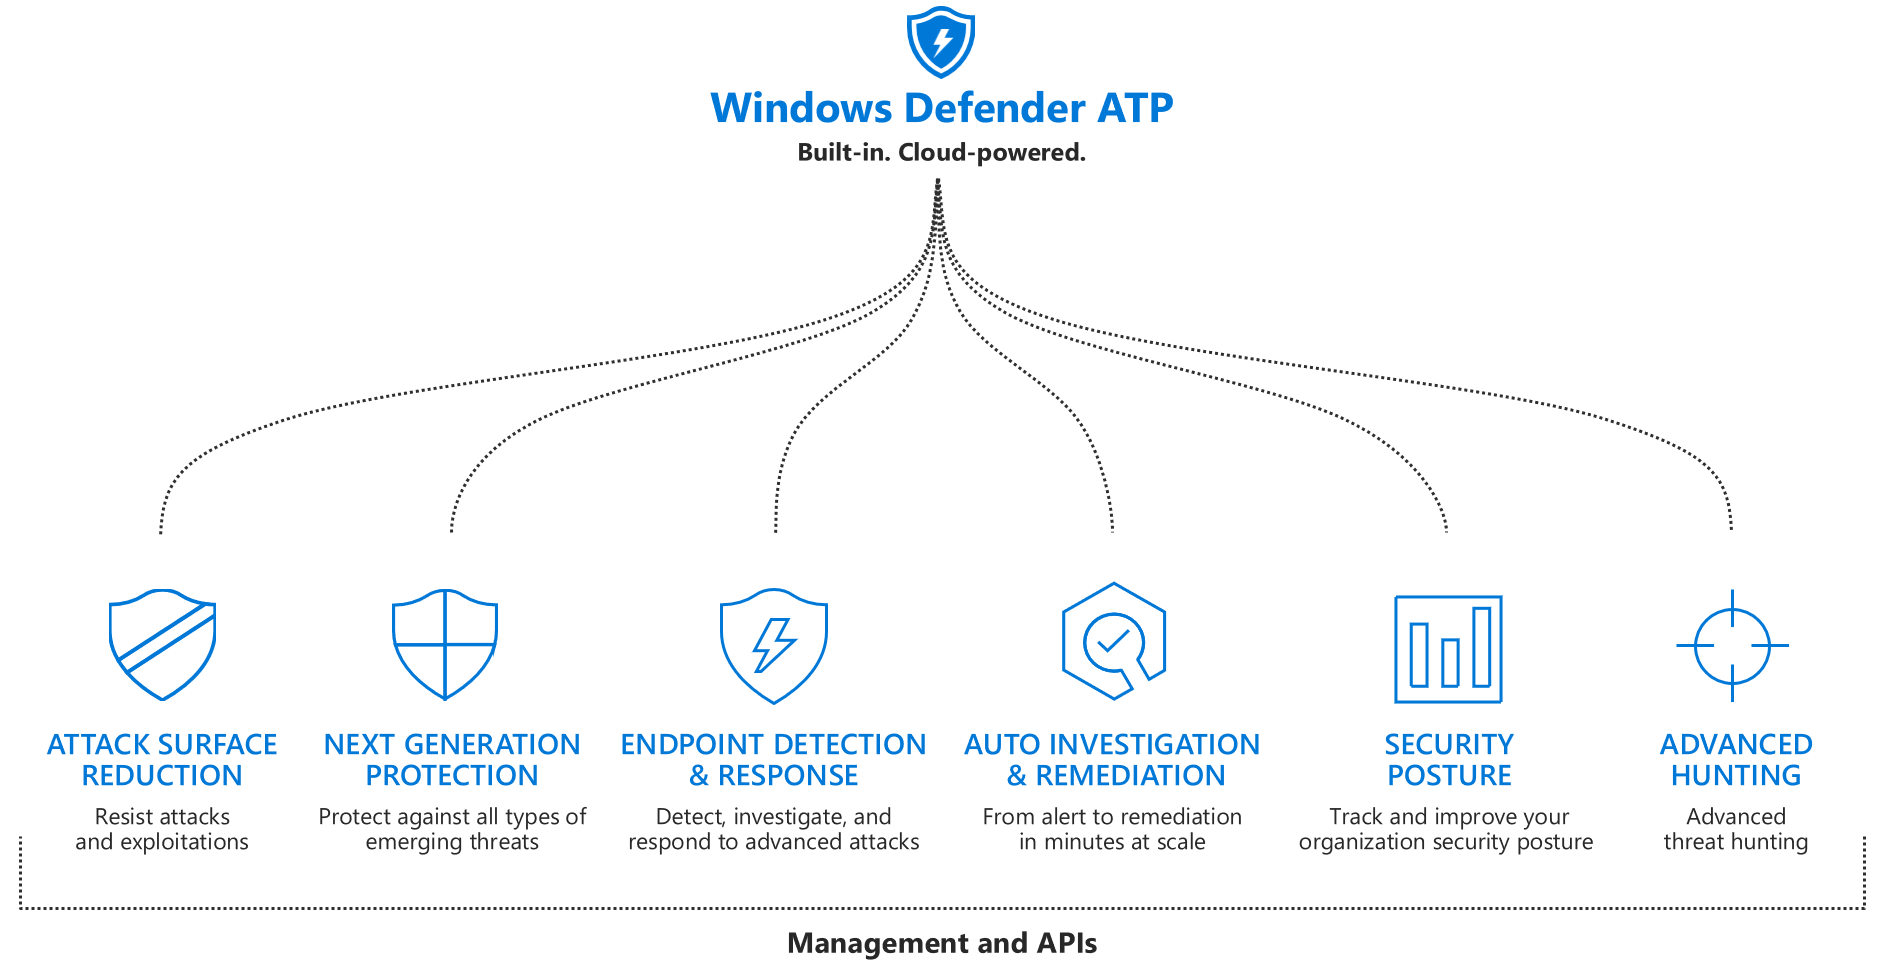
\includegraphics[width=\textwidth,height=6cm,keepaspectratio=true]{img/Windows-Defender-ATP.png}
	\caption{The picture above \autocite{WDATPT2018} shows the different components of Windows Defender \acrlong{atp}.}
	\label{fig:WDATPT2018}
\end{figure}
\subsubsection{Attack surface reduction}

\subsubsection{Next generation protection}
\subsubsection{Endpoint detection and response}
\subsubsection{Auto investigation and remediation}
\subsubsection{Security posture}
\subsubsection{Advanced hunting}

\subsection{Security with \acrfull{sdn}}
\subsection{Shielded Virtual Machines}

\section{Application platform}
%\subsection{Linux containers on Windows}
%\subsection{Building Support for Kubernetes}
%\subsection{Container improvements}
%\subsection{Encrypted Networks}
%\subsection{Network performance improvements for virtual workloads}
%\subsection{Low Extra Delay Background Transport}
%\subsection{Windows Time Service}
%\subsection{High performance SDN gateways}
%\subsection{New Deployment UI and Windows Admin Center extension for SDN}
%\subsection{Persistent Memory support for Hyper-V VMs}

\section{Hyper-converged infrastructure}